\subsection{Suivi de murs}
  On s'intèresse ici à la programmation d'un robot\footnote{Un robot en Lego
  Mindstorms NXT, nous ne disposons de plus que de deux capteurs à ultrasons et
  deux boutons poussoirs.} afin qu'il puisse longer un mur.

  Afin de longer un mur, on peut par exemple poser un capteur à ultrasons sur
  le côté gauche de notre robot. Lorsque nous détectons que nous sommes trop
  éloignés du mur, nous tournons légèrement à gauche.

  Cette méthode donnant des résultats peu probants si la direction initiale du
  robot n'est pas exactement parallèle au mur, on peut ajouter un autre capteur
  à ultrasons à l'avant du robot. Ainsi, on peut tourner désormais à gauche,
  tout en avançant légèrement, dès qu'on détecte que le mur est trop loin; et
  si on se retrouve face à notre mur, alors on tourne vers la droite jusqu'à ne
  plus l'être.

  Ainsi, on peut suivre un mur droit de manière assez régulière.

% le truc avant en parle un peu, et en l'état c'est pas français, pas clair...  
%  \subsubsection{Passage de l'extérieur d'un angle}
%    Le passage de l'extérieur d'un angle (i.e.\ quand un mur tourne à gauche)
%    se fait naturellement à partir du code pour longer d'un mur: il suffit de
%    tourner à gauche (tout en avançant, afin d'éviter les collisions avec les
%    murs) jusqu'à ce qu'on soit à nouveau à côté d'un mur. Naturellement, il
%    faut adapter les coefficients de tournage, afin d'éviter que le robot ne
%    prenne un angle trop large, et se retrouve finalement face au mur qu'il est
%    censé longer.

\subsection{Labyrinthe}\label{sec:laby}
  \subsubsection{Suivi de mur}
    Le suivi de mur est déjà un algorithme admissible pour la résolution de
    labyrinthe, il trouvera une solution s'il en existe une. L'algorithme de
    Dijkstra et l'algorithme A* (qui est considéré comme une extension de
    premier) sont utilisés pour trouver le chemin le plus court.

  \subsubsection{Algorithme de Dijkstra}
    L'algorithme de Dijkstra est un algorithme permettant de trouver le plus
    court chemin entre deux sommets d'un graphe (orienté ou non). Sa complexité
    est polynomiale.

    Son principe est simple : il parcourt le graphe en gardant en mémoire la
    longueur du chemin le plus court vers chaque sommet.

    \begin{algorithm}
      \KwIn{deux sommets s1 et s2}
      %\Require{il existe une chaine entre les deux sommets}
      \KwOut{le plus court chemin entre s1 et s2}
      \Begin{%
        \For{chaque sommet du graphe}{%
          sommet.parcouru $\leftarrow \infty$\;
          sommet.precedent $\leftarrow 0$\;
        }
        s1.parcouru $\leftarrow 0$\;
        non\_visités $\leftarrow$ ensemble des sommets du graphe\;

        \While{non\_visités est non vide}{%
          s $\leftarrow$ le sommet de non\_visités avec parcouru minimum\;
          supprimer s de non\_visités\;

          \For{chaque sommet f fils de s}{%
            \If{f.parcouru > s.parcouru + poids de l'arc entre s et f}{%
              f.parcouru $\leftarrow$ s.parcouru + poids de l'arc entre s et f\;
              f.precedent $\leftarrow$ s\;
              ajouter f dans non\_visités\;
            }
          }
        }

        chaine $\leftarrow$ liste vide\;
        s = s2\;
        \While{s $\neq$ s1}{%
          chaine.ajouter(s)\;
          s $\leftarrow$ s.precedent\;
        }

        chaine.ajouter(s1)\;
        \Return{chaine}
      }
      \caption{Algorithme de Dijkstra}
      \label{alg:dijkstra}
    \end{algorithm}

    % TODO : Améliorer ça, c'est pas ma partie..
    Cet algorithme est appliquable une fois qu'on a obtenu un graphe a partir du plan du labyrinthe.

    \begin{center}
      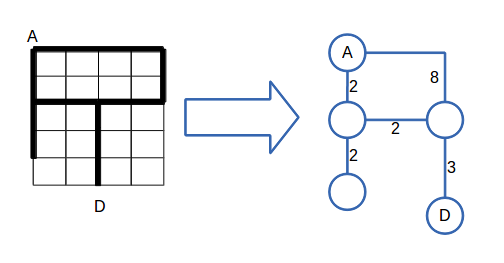
\includegraphics[width=0.55\textwidth]{../slides/jeux/GRO_graph1.png}
    \end{center}

    %todo: il n'y a pas de Dijkstra dans la partie graphes
    On peu appliquer l'algorithme de Dijkstra tel qu'il a été présenté dans la
    première partie "Graphes" à ce graphe et trouver le chemin le plus court.

  \subsubsection{Algorithme A*}
  % TODO: On met vraiment A* ? J'aurais un peu envie de dire OSEF...
    L'algorithme A* est une amélioration de Dijkstra, qui utilise une heuristique
    pour orienter la recherche.
    Si l'heuristique est bien choisi, il est même possible de s'assurer qu'A*
    donnera bien le résultat optimal (mais plus rapidement que Dijkstra).

    Cet algorithme utilise deux listes de nœuds: une liste, dite ouverte, qui
    contient les nœuds explorables et une liste, dite fermée, qui contient les
    nœuds déjà explorés.

    \begin{itemize}
      \item On crée un nœud en lui attribuant un cout heuristique qui
        correspond au cout du nœud plus une estimation de la distance de ce
        nœud à l'arrivée.

        Remarque: l'utilisation de ce cout heuristique est une différence
        notable avec l'algorithme de Dijkstra, elle permet de s'assurer que
        l'on va toujours plus ou moins dans la bonne direction.

        Par exemple dans un graphe en étoile avec des branches de même taille
        et plusieurs nœuds par branches ou l'on part du centre pour rejoindre
        l'extrémité d'une branche l'algorithme de Djkstra explore toutes les
        branches simultanément alors qu'avec l'utilisation du cout heuristique
        on explore directement et uniquement la bonne branche.
      \item On ajoute ce nœud à la liste ouverte.
      \item On prend le nœud qui a le meilleur cout heuristique dans la liste
        ouverte et on l'ajoute à la liste fermée.
      \item On crée les nœuds adjacents et pour chacun d'eux:
        \begin{itemize}
          \item Leur cout est égal à la somme des couts de leurs prédécesseurs
            et du cout entre les deux.
          \item Si l'un d'eux est présent dans la liste ouverte on vérifie si
            ce nouveau chemin trouvé est plus rapide. Si c'est le cas on
            remplace celui qui est dans la liste ouverte par le nouveau sinon
            on oublie le nouveau.
          \item S'il est déjà dans la liste fermée c'est qu'il a déjà été
            traité ou qu'il est en train d'être traité donc on l'oublie.
          \item Et si il n'est ni dans la liste ouverte ni dans la liste fermée
            on l'ajoute à la liste ouverte.
        \end{itemize}
    \end{itemize}
	
    À la fin, en remontant tous les prédécesseurs on remonte le chemin le plus
    court.

% vim: shiftwidth=2 softtabstop=2 tabstop=2
